\documentclass{article}

\usepackage{graphicx}
\usepackage{cite}
\usepackage{pdflscape}
\graphicspath{ {./images/} }
%Tarih Ekleme
\usepackage[ddmmyyyy]{datetime}
\renewcommand{\dateseparator}{.}
\renewcommand{\figurename}{Şekil}
\renewcommand{\refname}{Kaynakça}

\title{Yapay Zeka ile Sesten Yazıya Dönüştürme}
\author{Samet Duran}
\date{10.03.2024}
\begin{document}
	\maketitle
	\pagenumbering{gobble}
	\newpage
	\pagenumbering{arabic}
	\section{Giriş}
	Bu projede insanların konuşmalarının metne dönüştürülerek bilgisayar ortamına aktarılması amaçlandı bu yüzden yapay zeka ile sesten yazıya çevirme konusu seçildi. Bu konuda ki örnekler araştırıldı. Python dili kullanılmasına karar verildi. Openai şirketinin açık kaynak kodlu Whisper adlı modeli ve Mozilla şirketinin açık kaynak kodlu Deepspeech adlı modeli incelendi ve araştırıldı. Deepspeech modeli WHisper modeli ile karşılaştırıldı. Proje sonunda konuşmayı yazıya çeviren bir uygulama ortaya çıkacak.
	 
	\section{Literatür Araştırması}
	OpenAI'nin Whisper ile Mozilla'nın Deepspeech modelleri Konuşmadan Yazıya Dönüştürme konusunda geliştirilmiş modellerdir.
	
	\subsection{Genel Bilgi:}
	
	Konuşmadan yazıya (STT) dönüştürme, sesli konuşmayı metne dönüştüren bir teknolojidir.
	
	\subsection{Whisper:}
	\begin{itemize}
		\item Açık kaynaklı bir ASR modelidir.
		\item Şuanlık gerçek zamanlı şekilde çalışmıyor, ses dosyası yüklenerek çalıştırılabiliyor.
		\item Çok dilli bir konuşma tanıma sistemi olarak öne çıkar.
		\item 680.000 saatten fazla çok dilli ve webden toplanan veriyle eğitilmiştir.
		\item Bu büyük veri havuzu, benzersiz vurguları, arka plan gürültüsünü ve teknik jargonu daha iyi tanımasına olanak sağlar
		\item Whisper, hızlı ve doğru sonuçlar elde etmek için tasarlanmıştır.
	\end{itemize}
	
	\subsection{Deepspeech:}
		DeepSpeech DeepSpeech, Baidu'nun Deep Speech araştırma makalesine \cite{DBLP:journals/corr/HannunCCCDEPSSCN14} dayanan makine öğrenimi teknikleriyle eğitilmiş bir model kullanan açık kaynaklı bir Konuşmadan Metne motorudur. DeepSpeech Projesi, uygulamayı kolaylaştırmak için Google'ın TensorFlow 'unu kullanır. TenserFlow Google tarafından geliştirilen uçtan uca açık kaynaklı bir makine öğrenmesi kütüphanesidir.
	\begin{itemize}
		\item Mozilla tarafından geliştirilen bir ASR modelidir.
		\item Gerçek Zamanlı çalışıyor fakat sadece ingilizce destekliyor.
		\item Açık kaynaklı ve topluluk tarafından desteklenir. 
		\item Wav2Vec 2.0 gibi unsupervised training temelinde çalışır.
		\item Raw waveform representation, context part ve linear layer olmak üzere üç bölümden oluşur.
		\item Wav2Vec 2.0, konuşma tanıma alanında önemli bir başarıya sahiptir \\
	\end{itemize}
	Sonuç olarak Whisper gerçek zamanlı çalışmıyor fakat Deepspeech modeline göre çok daha doğru sonuçlar veriyor.
	
	
	\section{Sesten Yazıya Çevirmenin Metodolojisi}
	Whisper’ın mimari tasarımı basit ve etkilidir. Bir encoder-decoder Transformer olarak uygulanmıştır. İşlem adımları şu şekildedir:
	\begin{itemize}
		\item Giriş Sesinin Bölünmesi: Giriş sesi 30 saniyelik parçalara bölünür.
		\item Log-Mel Spektrogramına Dönüştürme: Her parça bir log-Mel spektrogramına dönüştürülür.
		Log Mel spektrogramı, ses işleme alanında yaygın olarak kullanılan bir görsel temsil yöntemidir. Bu yöntem, ses sinyallerinin frekans içeriğini zamanla nasıl değiştirdiğini görselleştirmek için kullanılır. \\ \\ Log Mel Spektogramı hakkında daha ayrıntılı açıklama:
		\subitem Ses Sinyali ve Örnekleme: Bir ses sinyali, zaman içinde belirli bir niceliğin değişimini temsil eder. Ses sinyalleri için bu nicelik hava basıncıdır. Ses sinyalini dijital olarak işlemek için zaman içinde hava basıncının örneklerini alabiliriz. Bu örnekleri almak için veri örnekleme hızı genellikle 44.1 kHz’dir (yani saniyede 44,100 örnek). Bu örnekleme işlemiyle, ses sinyalinin dijital bir temsilini elde ederiz.
		\subitem Fourier Dönüşümü: Ses sinyali, birçok tek frekanslı ses dalgasından oluşur. Zaman içinde sinyalin örneklerini alırken, sadece sonuç amplitüdlerini yakalarız. Fourier dönüşümü, bir sinyali frekans bileşenlerine ayırarak frekans alanına dönüştüren matematiksel bir formüldür. Bu, sinyali zamandan frekansa dönüştürür ve sonuç spektrum olarak adlandırılır. Her sinyal, orijinal sinyale toplamı veren bir dizi sinüs ve kosinüs dalgasına ayrılabilir. Bu, Fourier teoremi olarak bilinir.
		\subitem Hızlı Fourier Dönüşümü (FFT): FFT, Fourier dönüşümünü verimli bir şekilde hesaplayabilen bir algoritmadır ve sinyal işlemede yaygın olarak kullanılır. Örnek ses verisini FFT algoritmasıyla analiz edebiliriz. Bu, sinyalin frekans içeriğini incelememizi sağlar.
		\subitem Spektrogram: FFT, bir sinyalin frekans içeriğini analiz etmek için güçlü bir araçtır, ancak sinyalin frekans içeriği zamanla nasıl değişirse? Bu durum, müzik ve konuşma gibi çoğu ses sinyali için geçerlidir. Spektrogram, bu tür sinyallerin zaman içindeki spektrumunu temsil etmek için kullanılır. Log Mel spektrogramı, önce sinyalin Mel ölçeğindeki logaritmik güç spektrumunu hesaplar ve ardından bu spektrumu görselleştirir. Mel ölçeği, insan işitme algısına daha iyi uyan bir frekans ölçeğidir.
		\item Kodlayıcı (Encoder): Log-Mel spektrogramı kodlayıcıya iletilir. Kodlayıcı, giriş sesini temsil eden bir vektör oluşturur.
		\item Dekoder (Decoder): İlgili metin başlığını tahmin etmek üzere eğitilmiş bir dekoder kullanılır. Bu sırada tek bir modelin dil tanımlaması, ifade düzeyinde zaman damgaları, çok dilli konuşma transkripti ve İngilizce’ye çeviri gibi görevleri gerçekleştirmesi için özel belirteçlerle karıştırılır.
		\item Whisper, geniş ve çeşitli bir veri kümesi üzerinde eğitildiği için, farklı aksanlara, arka plan gürültüsüne ve teknik dil kullanımına daha iyi uyum sağlar. Ayrıca, birden fazla dilde transkript yapabilir ve bu dilleri İngilizce’ye çevirebilir.
	\end{itemize}
	

	\subsection{Sesten yazıya çevirme teknolojisinin kullanım alanları:}
	\begin{itemize}
		\item Toplantı ve ders notları alma
		\item Video ve ses dosyalarını metne dönüştürme
		\item Engelli kişilere erişilebilirlik sağlama
		\item Müşteri hizmetlerinde ve çağrı merkezlerinde
		\item Altyazı oluşturma
	\end{itemize}
	
	
	
	\section{VeriTabanı ve Veriler}
	DeepSpeech’in İngilizce modeli, öğrenme için LibriSpeech, Fisher ve Santral projelerinden gelen verileri içerir. Ayrıca, Common Voice adlı bir veri kümesi kullanılmıştır. Bu veri kümesi, yaklaşık 3816 saatlik transkripsiyonlu radyo programı kayıtlarını içerir.
	Ayrıca, DeepSpeech’in deneysel Mandarin Çince akustik modelleri de bulunmaktadır. Bu modeller, 2000 saatlik okuma metni içeren bir iç veri kümesi üzerinde eğitilmiştir. Bu modeller, bellek haritalı (“.pbmm” uzantılı) ve TensorFlow Lite kullanılarak dönüştürülmüş (“.tflite” uzantılı) olmak üzere iki farklı formatta sunulmaktadır.\\
	
	Mevcut diğer yaklaşımlar sıklıkla daha küçük, daha yakın eşleştirilmiş ses-metin eğitim veri kümeleri kullanmakta,\cite{DBLP:journals/corr/abs-2104-02133}, \cite{DBLP:journals/corr/abs-2111-09344},\cite{DBLP:journals/corr/abs-2106-06909} veya geniş ancak denetimsiz ses ön eğitimi kullanmaktadır.\cite{DBLP:journals/corr/abs-2006-11477}, \cite{Zhang_2022} Whisper büyük ve çeşitli bir veri kümesi üzerinde eğitildiği ve herhangi bir veri kümesine göre ince ayar yapılmadığı için, konuşma tanıma alanında rekabetçi bir ölçüt olarak bilinen LibriSpeech performansında uzmanlaşmış modelleri geçememektedir. Bununla birlikte, Whisper'ın sıfır atış performansını birçok farklı veri kümesinde ölçtüğümüzde, çok daha sağlam olduğunu ve bu modellerden %50 daha az hata yaptığını görüyoruz.
	Whisper'ın ses veri kümesinin yaklaşık üçte biri İngilizce değildir ve dönüşümlü olarak orijinal dilde yazıya dökme veya İngilizceye çevirme görevi verilir. Bu yaklaşımın özellikle konuşmadan metne çeviriyi öğrenmede etkili olduğunu ve CoVoST2'deki denetimli SOTA'dan İngilizce çeviriye sıfır atışta daha iyi performans gösterdiğini görüyoruz.
	
	\section{Proje planlama Gantt Çizelgesi}
	\begin{figure}[!htbp]
		\caption{GANTT ÇİZELGESİ}
		\centering
		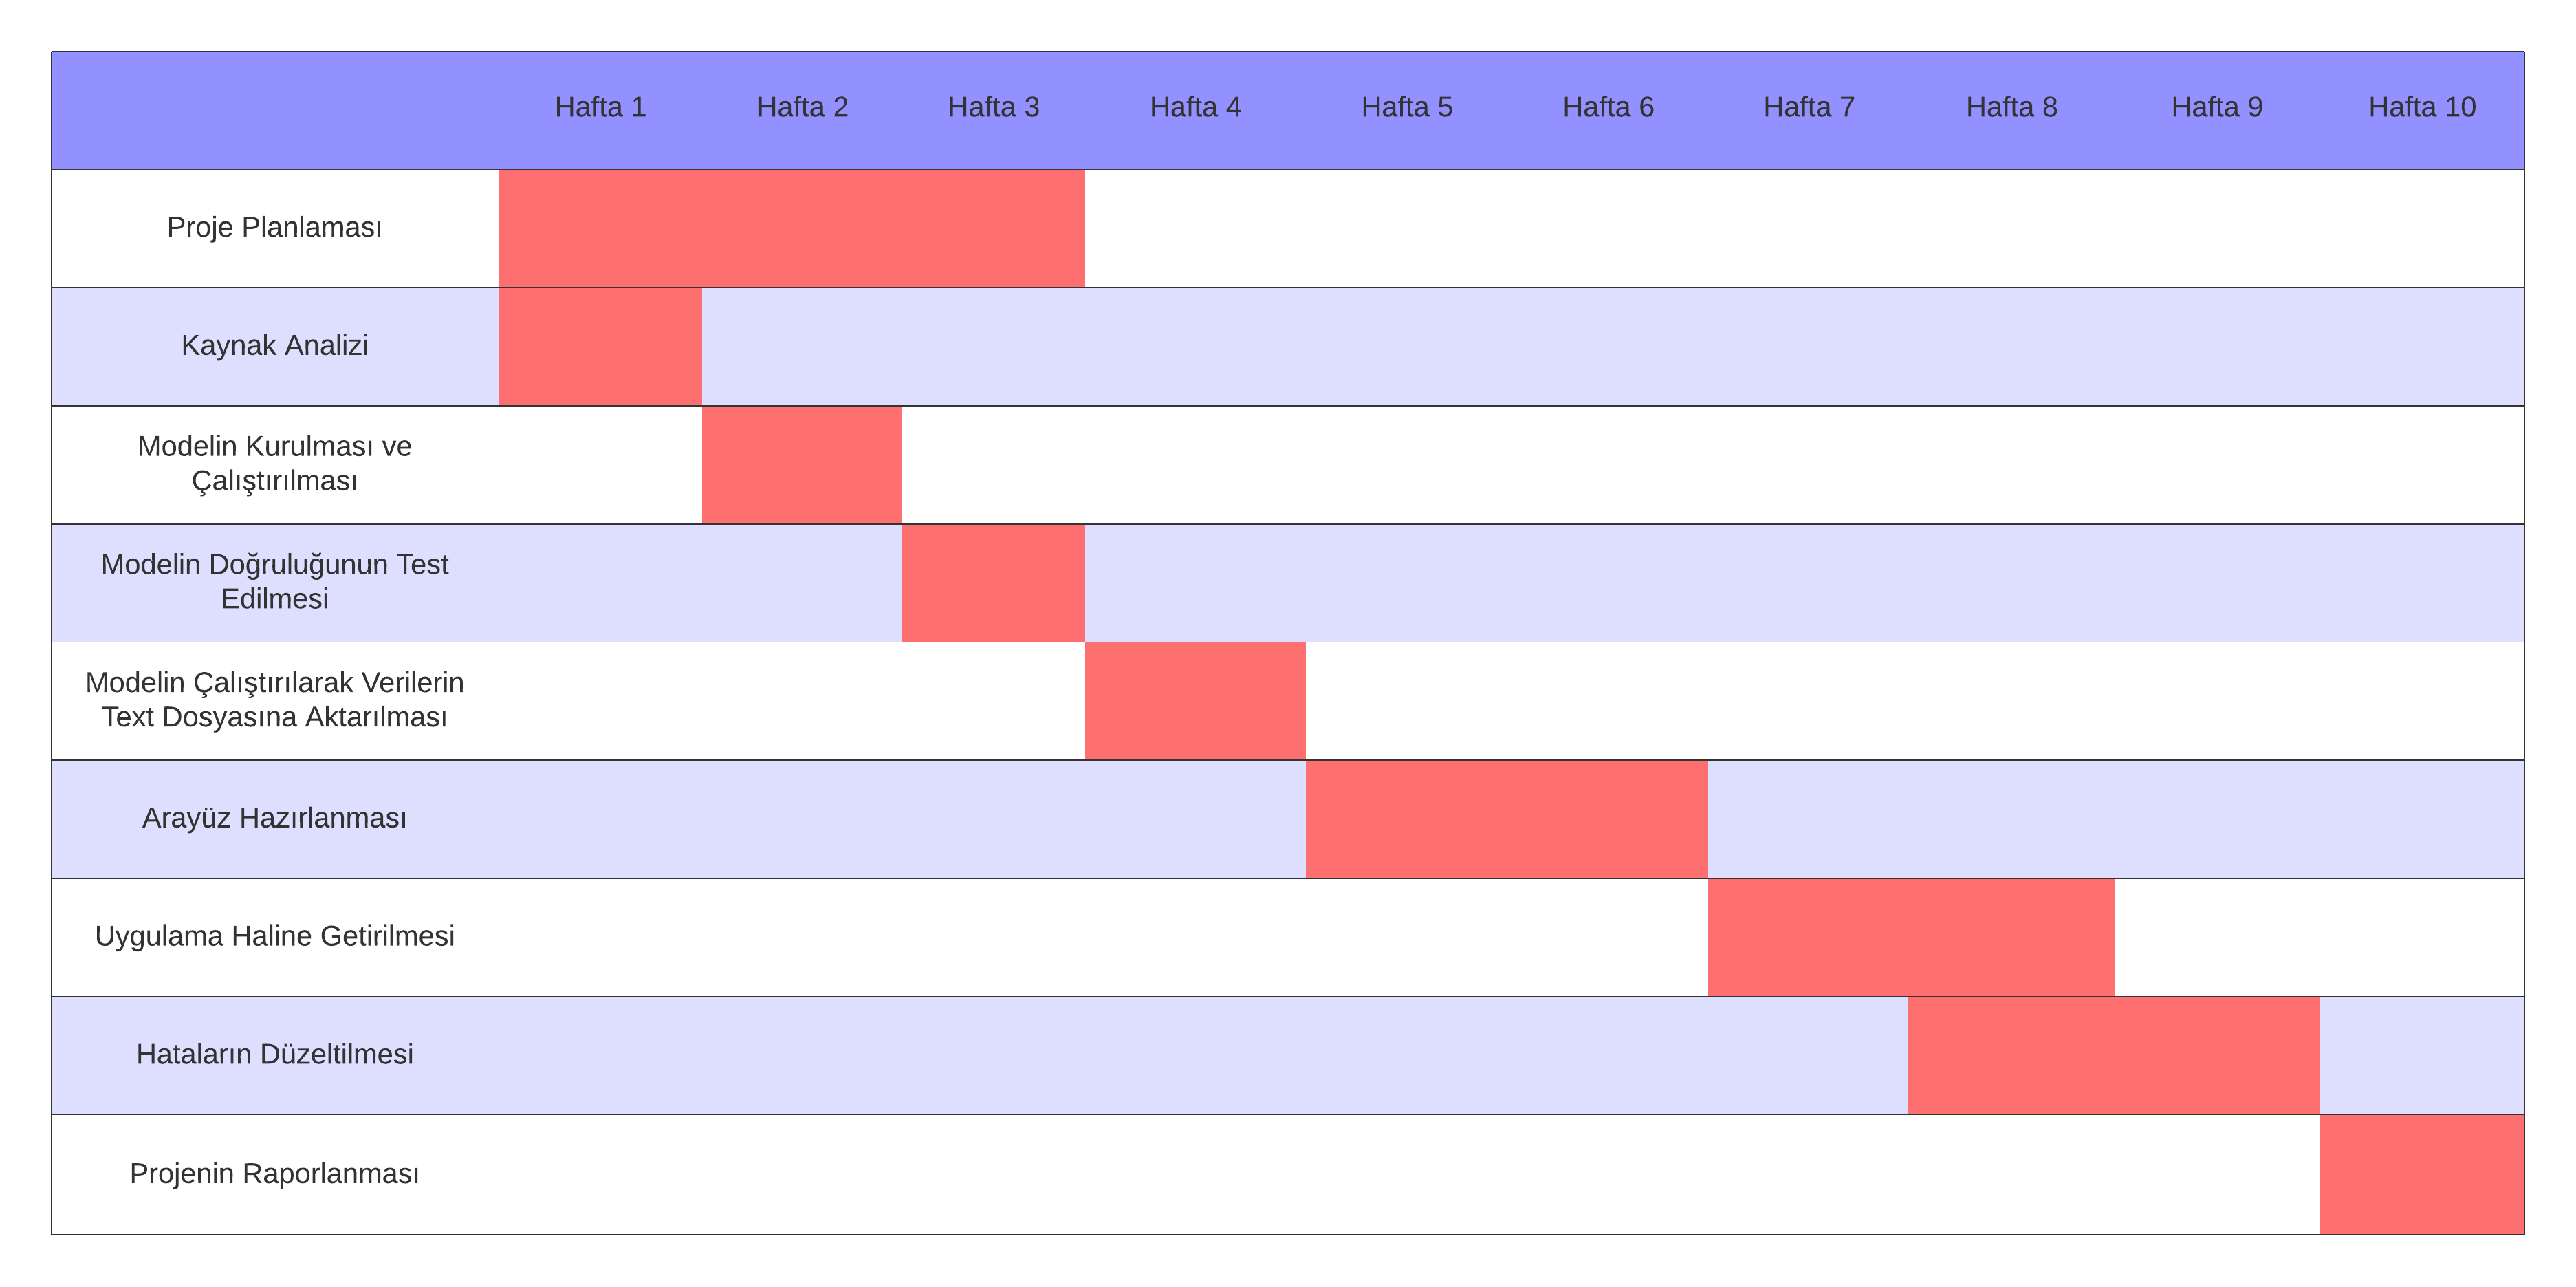
\includegraphics[width=15cm,
		height=6cm,
		keepaspectratio]{ganttchart.png}
		\label{gantt}
	\end{figure}
	\newpage
	
	

\bibliographystyle{ieeetr}
\bibliography{./references} 
	\begin{itemize}
		\item https://towardsdatascience.com/speech-to-text-with-openais-whisper-53d5cea9005e
		\item https://github.com/openai/whisper
		\item https://openai.com/research/whisper
		\item https://medium.com/analytics-vidhya/understanding-the-mel-spectrogram-fca2afa2ce53
		\item https://blog.desdelinux.net/tr/derin-konu%C5%9Fma-mozilla-konu%C5%9Fma-tan%C4%B1ma-motoru/
		\item https://github.com/mozilla/DeepSpeech/releases
	\end{itemize}
\end{document}